\chapter{MODELO DE VELOCIDADES COM VARIAÇÃO LATERAL}
\label{cap11}

Esta etapa do desenvolvimento da tese ainda não está totalmente concluída. Neste capítulo apresentamos
os resultados preliminares:
A segunda etapa da estratégia de inversão do modelo de velocidades consiste em encontrar a perturbação
$\delta v(x,z)$ para um modelo de velocidades de background arbitrário.
Utilizamos o modelo de velocidades de gradiente constante (Figura \ref{fig:10.2} à direita)
obtido na etapa de inversão do Capítulo 10. O objetivo desta etapa é obter a correta 
localização das fontes PIN sobre os refletores do modelo de velocidades original (Figura \ref{fig:9.2}).
Assim, definimos o novo modelo de velocidades com variação lateral de velocidade na
Equação a seguir:

\begin{equation}
\label{eq:11.1}
v(x,z)=z g_z+v_0+\delta v(x,z)
\end{equation}

Onde $z$ é a coordenada da profundidade, $g_z$ é o gradiente de velocidades em profundidade obtido na
etapa de inversão anterior e $v_0$ é a velocidade próxima da superfície. O termo $\delta v(x,z)$ representa
a perturbação no modelo de velocidades de background (Equação \ref{eq:10.1})
representado pelas duas primeiras parcelas à direita na 
Equação \ref{eq:11.1}.

A otimização do modelo de velocidades
representado pela Equação \ref{eq:11.1}
é realizada de forma semelhante à desenvolvida no Capítulo 10:
Utilizamos a Equação \ref{eq:9.2} da soma das diferenças nos tempos de trânsito obtidos com o traçamento de raios no modelo de velocidades e os tempos de trânsito calculados utilizando a fórmula do ERC
(Equação \ref{eq:9.1}) como critério de convergência.
Todavia, nesta etapa, o algoritmo Very Fast Simulated Annealing (VFSA) é utilizado para realizar a otimização das perturbações $\delta v(x,z)$ do modelo de velocidades ao invés do gradiente de velocidades em
profundidade, já obtido na etapa anterior. Estas perturbações são atualizadas a cada iteração do VFSA (Ver a estratégia completa na representação esquemática do algoritmo na Figura \ref{fig:11.1}).

Ainda precisamos escolher a melhor estratégia para a representação do modelo de velocidades
e para a interpolação dos pontos sobre a malha. Temporariamente, utilizamos a representação
das perturbações do modelo de velocidades de background em uma malha regular de pontos de
controle $\Delta v_{ij}$. Somamos estas perturbações ao modelo de background nos pontos sobre
a malha utilizando a Equação \ref{eq:11.1} e interpolamos para todo o modelo de velocidades
através da interpolação essentially non-oscillatory (ENO) \cite{eno1,eno2}. Esta metodologia
de interpolação é utilizada para restringir o número de parâmetros a serem otimizados pelo VFSA
aos pontos de controle ao invés de otimizar todos os pontos sobre a malha do modelo de velocidades,
pois um número grande de parâmetros pode prejudicar a otimização com o VFSA.

\begin{figure}[H]
\caption{Representação esquemática do algoritmo de inversão do modelo de velocidades
com variação lateral de velocidade.}
\begin{center}
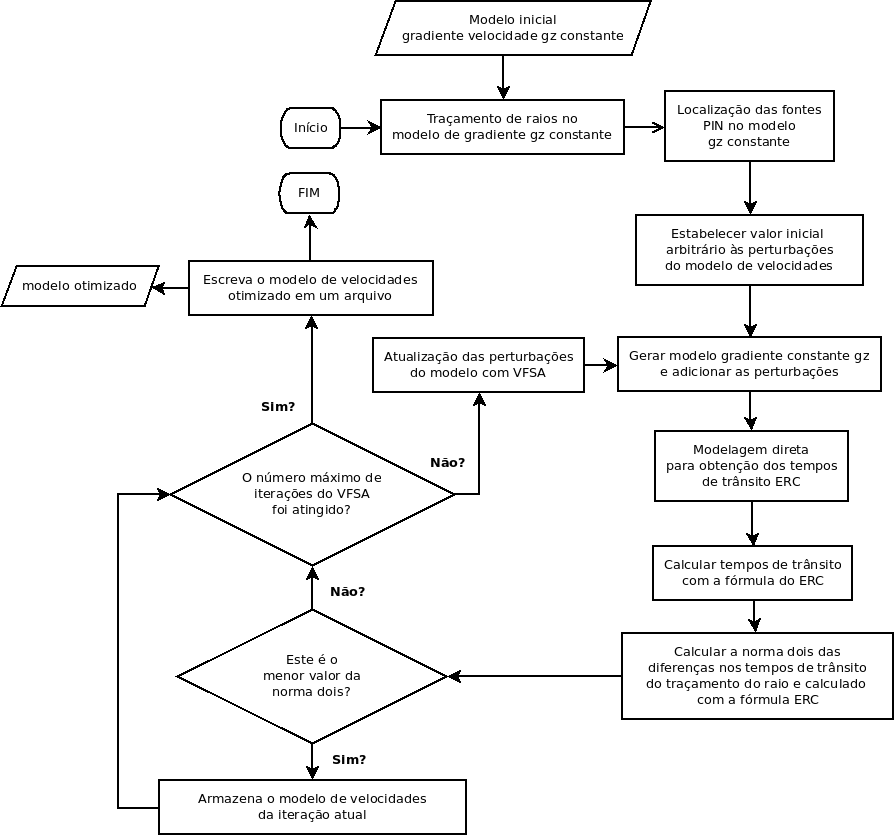
\includegraphics[scale=0.5]{images/fluxoinv.png}
\vspace{-0.3cm}
\end{center}
\begin{center}
 Fonte: Do Autor.
\end{center}
\label{fig:11.1}
\end{figure}

Assim, a Equação \ref{eq:11.1} se torna, para os nós da malha de pontos de controle:

\begin{equation}
\label{eq:11.2}
v_{ij}(x_j,z_i)=z_i g_z+v_0+\delta v_{ij}
\end{equation}

Deste modo, a estratégia de inversão do modelo de velocidades consiste em obter
as perturbações $\delta v_{ij}$ do modelo de velocidades de background (Equação \ref{eq:11.2})
de modo a produzir a melhor localização das fontes PIN sobre os refletores em profundidade.
A velocidade próxima à superfície $v_0$ e o gradiente de velocidades $g_z$ são constantes conhecidas
e definem o modelo de velocidades de background.

\begin{figure}[H]
\caption{Resultado da inversão do modelo de velocidades. Houve considerável melhora na
localização das fontes PIN (cruzes em preto) sobre os refletores em profundidade.}
\begin{center}
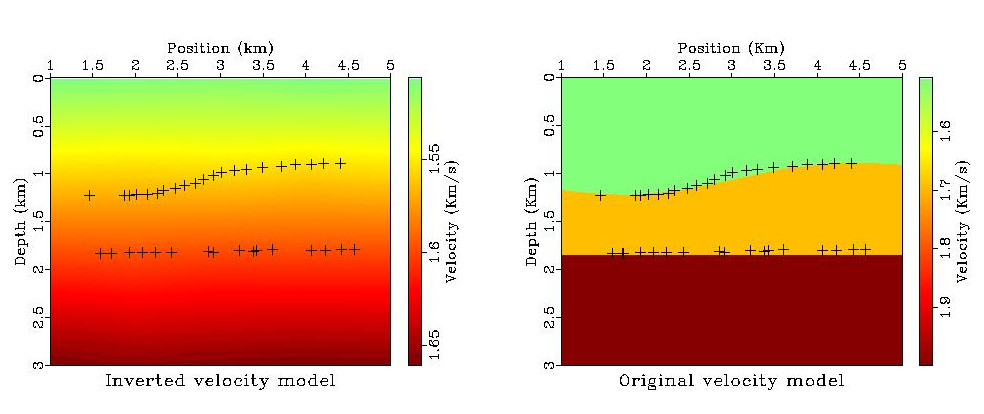
\includegraphics[scale=2]{images/inverted-original.jpeg}
\vspace{-0.3cm}
\end{center}
\begin{center}
 Fonte: Do Autor.
\end{center}
\label{fig:11.2}
\end{figure}

\begin{figure}[H]
\caption{Resultado da localização das fontes PIN (cruzes em preto)
para o modelo de velocidades de gradiente constante sobre o modelo de velocidades original.}
\begin{center}
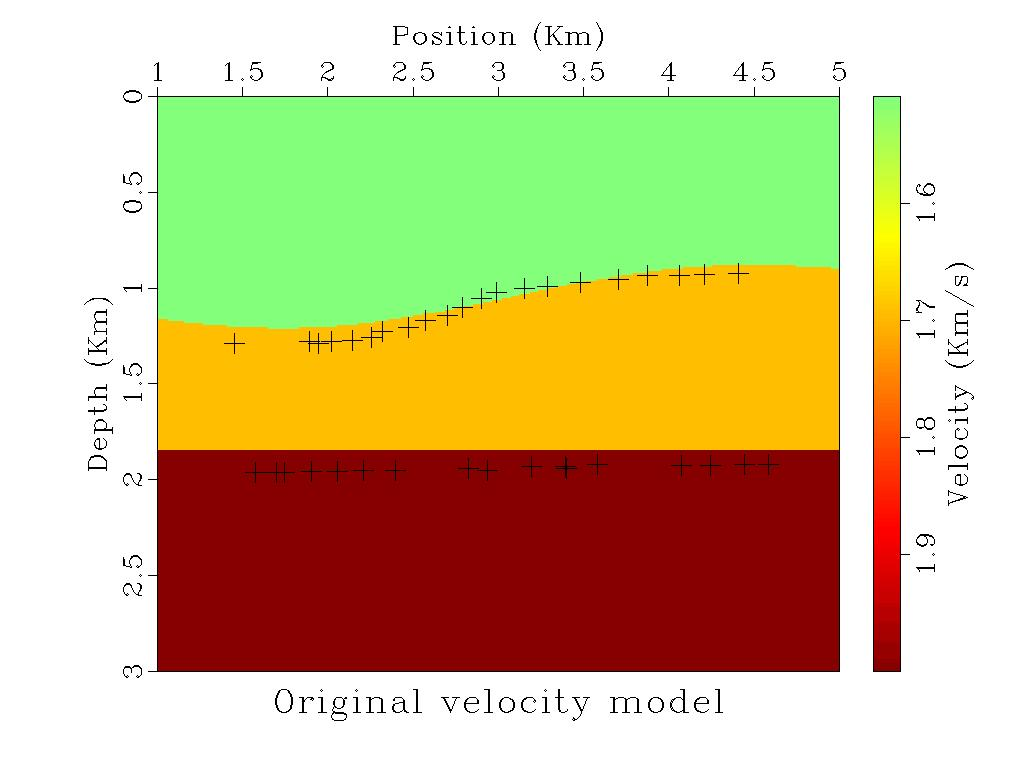
\includegraphics[scale=0.25]{images/gzvel.jpeg}
\vspace{-0.3cm}
\end{center}
\begin{center}
 Fonte: Do Autor.
\end{center}
\label{fig:11.3}
\end{figure}

\begin{figure}[H]
\caption{Resultado da localização das fontes PIN (cruzes em preto)
para o modelo de velocidades com perturbação sobre o modelo de velocidades original.}
\begin{center}
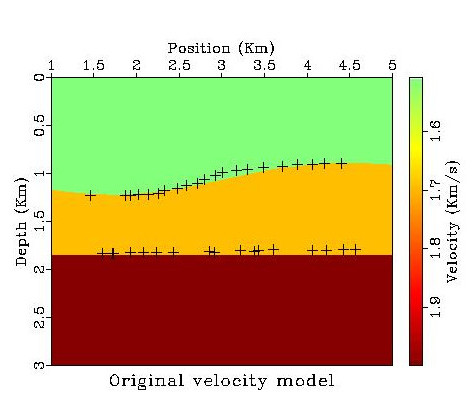
\includegraphics[scale=2.1]{images/endresult.jpeg}
\vspace{-0.3cm}
\end{center}
\begin{center}
 Fonte: Do Autor.
\end{center}
\label{fig:11.4}
\end{figure}

O resultado desta estratégia de otimização do modelo de velocidades é apresentado na Figura \ref{fig:11.2}.
Houve considerável melhora na localização das fontes pontuais PIN sobre os refletores (Ver
Figura \ref{fig:11.4}) em comparação com a etapa anterior do modelo de velocidades de
gradiente constante (Figura \ref{fig:11.3}).
Estes resultados indicam que a estratégia de inversão do modelo de velocidades utilizada é promissora, porém
que precisa ser elaborada uma melhor estratégia para a interpolação dos pontos sobre a malha do modelo de
velocidades e para suavizar o modelo (Figura \ref{fig:11.4}).
